\documentclass{scrartcl}

\usepackage[ngerman]{babel}

\usepackage[margin=0cm]{geometry}
\usepackage[hidelinks]{hyperref}
\usepackage{csquotes}

\usepackage{fontspec}
\setsansfont{TeX Gyre Heros}
\usepackage{fontawesome}

\usepackage{tikz}
\usetikzlibrary{calc}

\usepackage{graphicx}
\usepackage{xcolor}

\definecolor{fsfw-cyan}{HTML}{28ADB8}
\definecolor{fsfw-violett}{HTML}{654BC7}
\definecolor{fsfw-green}{HTML}{6BBB00}

\usepackage[outline]{contour}
\contourlength{0.05em}

\begin{document}

\begin{tikzpicture}[overlay,remember picture]
  
  % background
  \foreach \i in {-1,0,1,2,3,4,5} {
    \node[anchor=north,overlay]
    at ($(current page.north) + (0.07,0) + (2.258*\i, 5.65*-\i)$) {
      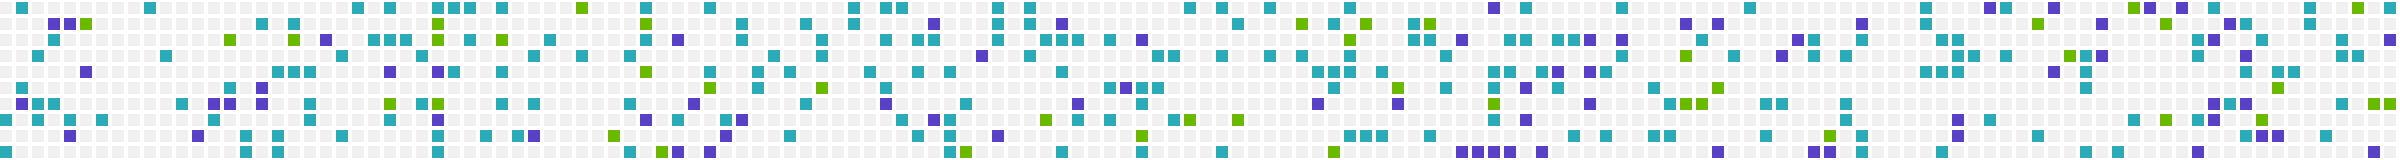
\includegraphics{banner.png}
    };
  }
  
  % top
  \node[anchor=north,fill=white,inner sep=0cm]
  at ($(current page.north) + (0,-1.31)$)
  {
    \begin{tikzpicture}
      \useasboundingbox[clip] (-9.53,5) rectangle (9.53,-5.1);
      \node[overlay] at (0,5)
      {
\includegraphics[width=30cm,origin=b]{book.jpg}};
      \node[scale=3,at={(-0.5,4)}]{%
        \contour{white}{\textbf{\textsf{\color{fsfw-cyan}\large%
              Schöne Abschlussarbeiten?}}}
      };
      \node[scale=3,at={(0,1.5)}]{%
        \contour{white}{\textbf{\textsf{\color{fsfw-violett}\Huge%
            Mit \LaTeX!}}}};
      \node[scale=3,at={(2,-2)}]{%
        \contour{white}{%
          \textbf{\textsf{\large\textcolor{fsfw-cyan}{%
                \dots{} aber es klappt nicht?}}}}};
      \node at (5,-4.3) {%
        \parbox{8cm}{\raggedleft%
          \tiny\sf \enquote{book} von walknboston, lizenziert unter CC-BY~2.0\\
          \url{https://www.flickr.com/photos/walkn/7454316418/}}};
    \end{tikzpicture}
  };


  % middle
  \node[fill=white,anchor=north,inner sep=0cm]
  at ($(current page.center) + (0,2.25)$){
    \begin{tikzpicture}
      \useasboundingbox (-9.53,5.75) rectangle (9.53,-5.5);
      \node[anchor=north] at (0,5.7) {
        \parbox[t][11.25cm][t]{18cm}{
          \begin{center}
            \Huge\color{fsfw-violett}
            \textbf{\textsf{\LaTeX/LibreOffice Helpdesk}}\\[1ex]
            \LARGE
            \color{black}
            \textsf{Direkte Hilfe bei Problemen mit \LaTeX{} und LibreOffice.}
          \end{center}

          \bigskip
          \bigskip

          \centering

          \parbox[t][6cm]{8cm}{
            {\Huge\textbf{\textsf{\textcolor{fsfw-green}{Termine}}}}

            \LARGE
            \null\quad\parbox{0.8\linewidth}{\sf%
              Mittwoch, 28.10.2015\\
              Mittwoch, 25.11.2015\\
              Mittwoch, 27.01.2016\\
              Mittwoch, 24.02.2016\\
              Mittwoch, 23.03.2016
            }
          }
          \parbox[t][6cm]{6cm}{
            \parbox[t][3.045cm]{\linewidth}{
              {\Huge\textbf{\textsf{\textcolor{fsfw-green}{Ort}}}}

              \vspace*{\baselineskip}

              \LARGE
              \quad\textsf{SLUB, Raum -2.115}
            }\\
            \parbox[t][3.5cm]{\linewidth}{
              {\Huge\textbf{\textsf{\textcolor{fsfw-green}{Zeit}}}}

              \vspace*{\baselineskip}

              \LARGE
              \quad\textsf{ab 19:00 Uhr}
            }
          }

          \vfill

          \begin{center}
            \large
            \textbf{\textsf{%
                \faicon{home}\,
                \url{https://fsfw-dresden.de/sprechstunde} \quad
                \faicon{envelope-o}\,
                \href{mailto:sprechstunde@fsfw-dresden.de}
                {\texttt{sprechstunde@fsfw-dresden.de}}}
            }
          \end{center}
        }
      };
    \end{tikzpicture}
  };
  
  % footer
  \node[anchor=south,fill=white,inner sep=0cm]
  at ($(current page.south) + (0,0.7)$) {\textbf{\textsf{
    \begin{tikzpicture}
      \useasboundingbox (-9.53,2) rectangle (9.53,-2);
      \node[rectangle,minimum height=3.5cm,minimum width=19cm] at (0,-2){
        \parbox[b][3.5cm]{4.5cm}{
          \null\vfill\centering
          
\includegraphics[origin=cc,width=4cm]{sitelogo.pdf}
          \vfill\null
        }
        \parbox[b][3.5cm]{14cm}{
          \null\vfill
          \centering
          \LARGE
          Hochschulgruppe für\\
          \Huge
          Freie Software und Freies Wissen\\
          \Large
          \medskip
          \url{https://fsfw-dresden.de}
          \vfill\null
        }
      };
    \end{tikzpicture}
  }}};
\end{tikzpicture}

\newpage

\end{document}

%%% Local Variables:
%%% mode: latex
%%% TeX-master: t
%%% TeX-engine: luatex
%%% End:
